\section{Udvikling af programmet}
	\subsection{Arkitektur}
		\begin{frame}[t]{Arkitektur}\framesubtitle{MVC \& Komponenter}
			\begin{columns}[T]
				\begin{column}{.48\textwidth}
					\begin{itemize}
						\item Client--Server arkitektur
						\item MVC
						\begin{itemize}
							\item Model
							\item View
							\item Controller
						\end{itemize}
						\item Komponent opdelt
						\item Data fra ekstern API
					\end{itemize}

				\end{column}
				\begin{column}{.48\textwidth}
					\begin{figure}
						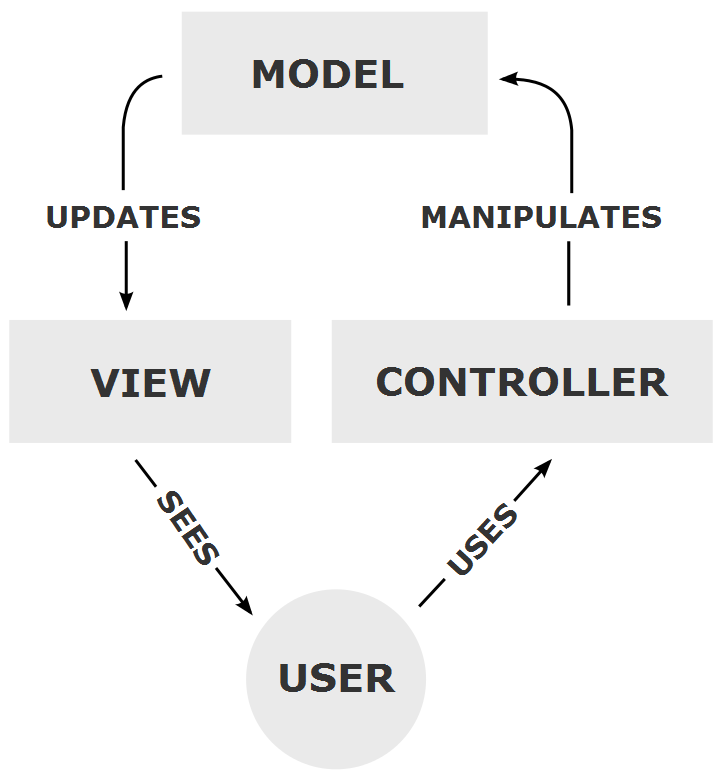
\includegraphics[width=1\textwidth]{images/MVC_2.png}
						\caption{MVC, figur af RegisFrey fra \url{wikipedia.org}}
					\end{figure}
				\end{column}
			\end{columns}
		\end{frame}
		
		\subsubsection{Funktionskomponenter}
		\begin{frame}[t]{Arkitektur}\framesubtitle{Funktionskomponenter}
			Komponenter har adgange og afhængighedder til hinanden
			%Topologisk sortering -> omvend reækkefølge -> implementer
			%Bruger > Tilbud > Indkøbsliste > Overvågning > Opskrift
			\hspace{-20pt}
			\begin{figure}[h!]
				\centering
				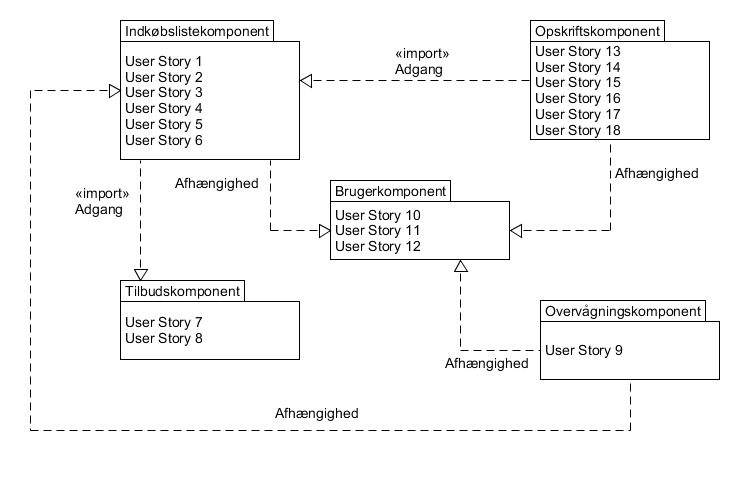
\includegraphics[width=1\textwidth]{images/Komponenter.png} % trim=1.4cm 6.1cm 6.5cm 1.8cm, clip, 
			\end{figure}
		\end{frame}

		\subsubsection{Modellag}
			\begin{frame}[t]{Arkitektur}\framesubtitle{Modellag}
				\begin{columns}[T]
				
					\begin{column}{.48\textwidth}
					\vspace{-29pt}
						\begin{figure}[h!]
							\centering
							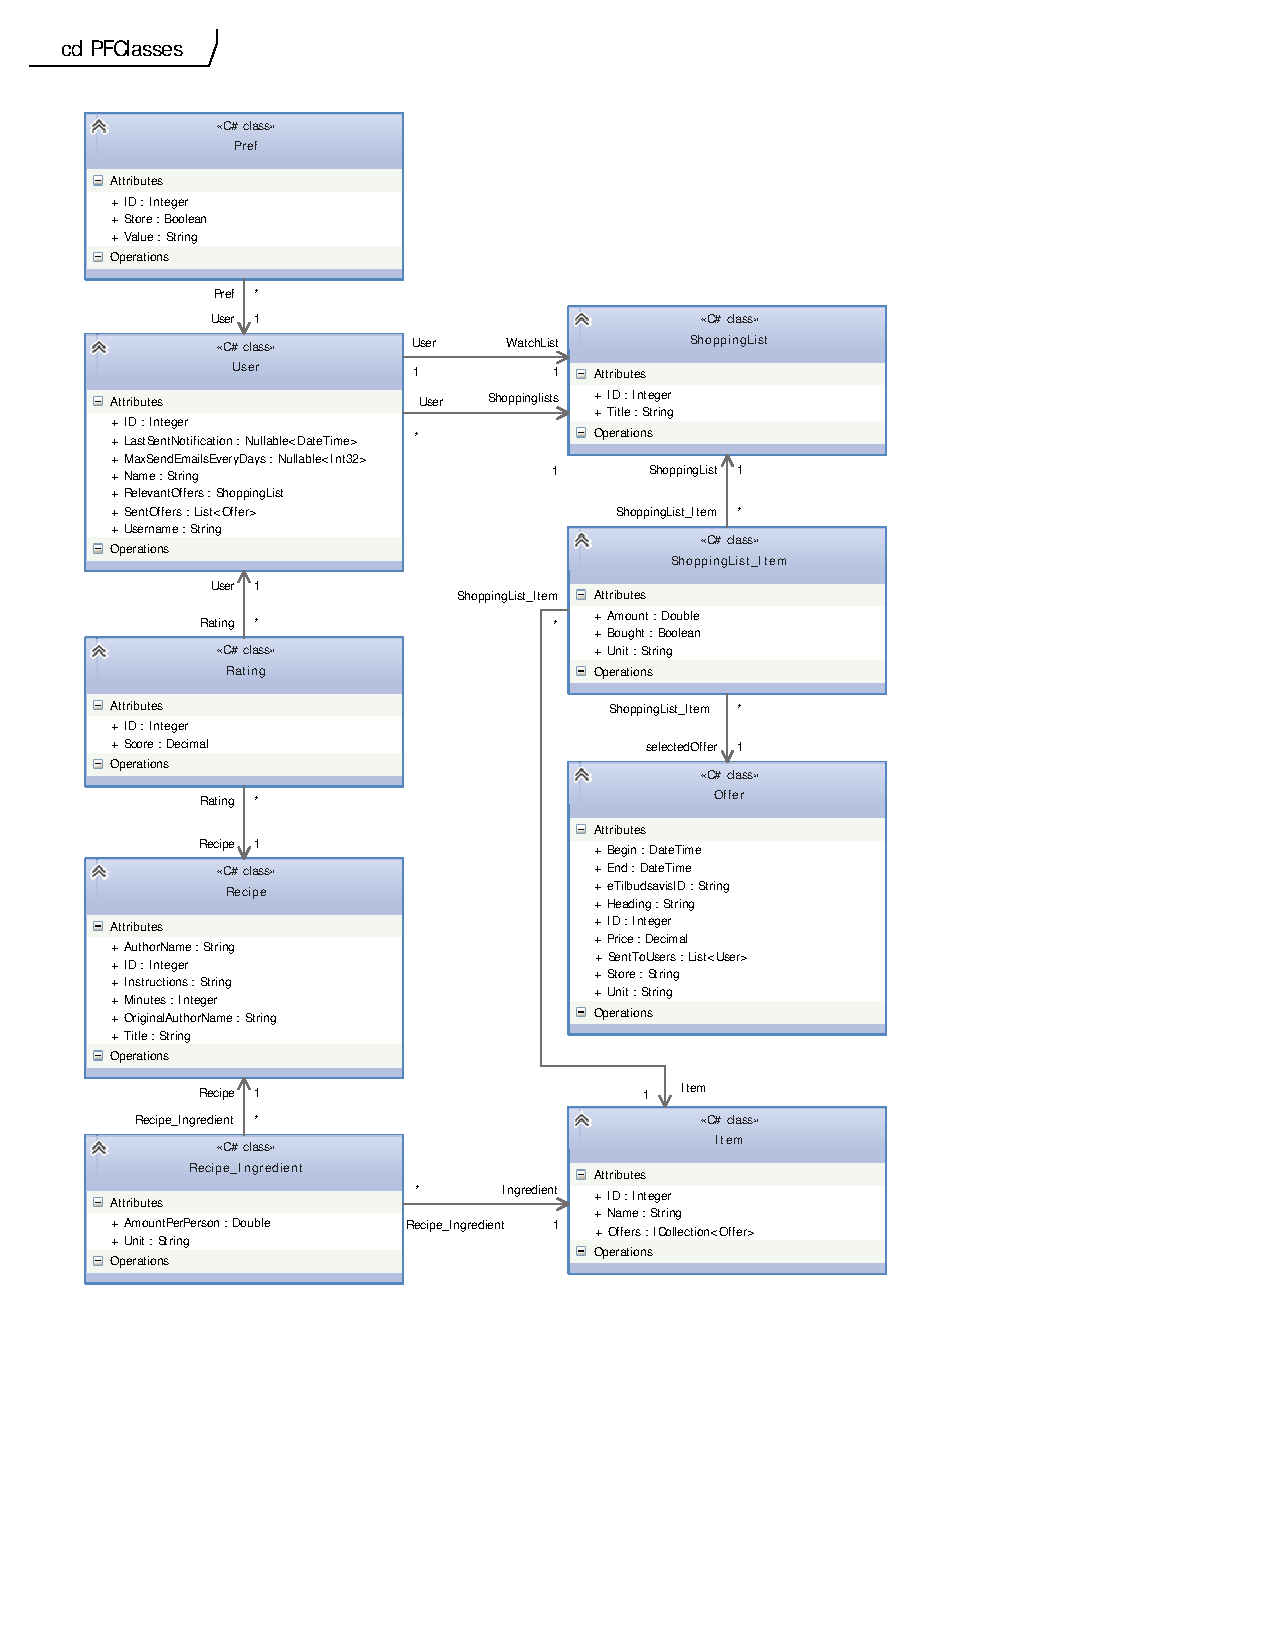
\includegraphics[trim=1.4cm 6.1cm 6.5cm 1.8cm, clip, width=1.125\textwidth]{images/PFClasses_2.pdf} % trim=1.4cm 6.1cm 6.5cm 1.8cm
						\end{figure}
					\end{column}
					\begin{column}{.44\textwidth}
						\begin{itemize}
							\item Implementering
							\item Iterationer
						\end{itemize}
					\end{column}
				\end{columns}
			\end{frame}

		\subsection{Teknologier}
			\begin{frame}[t]{Teknologier} %\framesubtitle{Udvikling intro}
				\begin{itemize}
					\item ASP.NET
					\begin{itemize}
						\item MVC
						\item Razor view engine
						\item Login system
					\end{itemize}
					\item Entity Framework
					\begin{itemize}
						\item Object--relational mapping
						\item Code--first
						\item Migrations
					\end{itemize}
					\item Bootstrap
					\begin{itemize}
						\item Responsiv layout
						\item CSS--klasser og JS
					\end{itemize}
				\end{itemize}
			\end{frame}

		\subsection{eTilbudsavis API}
			\begin{frame}[t]{Teknologier} \framesubtitle{eTilbudsavis API}
			Kommunikation med API'en:
				\begin{enumerate}
					\item POST api.etilbudsavis.dk/v2/\textbf{sessions}?api\_key=[...]
					\begin{itemize}
						\item Modtag \texttt{token}
						\item Beregn \texttt{signature} (SHA-256)
					\end{itemize}
					\item GET api.etilbudsavis.dk/v2/\textbf{offers}?r\_lat=57\&r\_lng=9
					\begin{itemize}
						\item Modtager 100 tilbud som JSON
						\item Gentages til alle er modtaget (do..while)
						\item Konverteres til \texttt{Offer}--klassen
					\end{itemize}
				\end{enumerate}
				\begin{itemize}
					\item Er tidskrævende (60-300 sekunder)
					\item Kan muligvis paralelliseres for bedre hastighed
					\item Dataet kunne være bedre
					\item Bliver filteret inden visning
				\end{itemize}
			\end{frame}